\documentclass[10pt,pdf,hyperref={unicode}]{beamer}
\usetheme{goettingen}
\usecolortheme{default}
\usefonttheme[onlymath]{serif}
\usepackage{bookmark}
\usepackage[utf8]{inputenc}
\usepackage[T2A]{fontenc}
\usepackage[english,russian]{babel}
\usepackage{graphicx}
\graphicspath{ {./images/} }

\title[Разработка модулей оповещения и статистики для системы дистанционного обучения]{\normalsize ВЫПУСКНАЯ КВАЛИФИКАЦИОННАЯ РАБОТА\\на тему: <<Разработка модулей оповещения и статистики для системы дистанционного обучения>>}
\author[Абдуллаева Е.]{\small Абдуллаева Евгения Гасановна}
\institute{\small Научный руководитель\\к.ф.-м.н., в.н.с. Алисейчик Павел Александрович}
\date{\small Ташкент 2021 г.}

\begin{document}
\begin{frame}
    \titlepage
\end{frame}

\begin{frame}{Содержание}
    \tableofcontents
\end{frame}

\section{Модуль оповещения}
\subsection{Подписка на оповещения}
\begin{frame}{Подписка на оповещения}
    \begin{figure}
        
\includegraphics[scale=0.4]{subscribe-button}
        \caption{Интерфейс подписки на оповещения о событиях курса}
        \centering
    \end{figure}
\end{frame}
\subsection{Оповещения о событиях на сайте}
\begin{frame}{Оповещения о событиях на сайте}
    Для пользователей реализована возможность получать оповещения о следующих событиях:
    \begin{itemize}
        \item о добавлении комментария;
        \item о новой посылке к задаче;
        \item о публикации объявления;
        \item о добавлении расписания;
        \item о создании вопроса;
        \item о сообщении об ошибке.
    \end{itemize}
\end{frame}
\subsection{Список оповещений}
\begin{frame}{Список оповещений}
    \begin{itemize}
        \item Бесконечная прокрутка списка оповещений
        \item Динамическая отметка оповещений как прочтенных при просмотре
    \end{itemize}
\end{frame}
\subsection{Интерфейс настройки оповещений}
\subsubsection{Выбор типов оповещений}
\begin{frame}{Выбор типов оповещений}
    \begin{figure}
        
\includegraphics[scale=0.4]{activity-settings}
        \caption{Интерфейс настройки оповещений: выбор типов оповещений}
        \centering
    \end{figure}
\end{frame}
\subsubsection{Список подписок на курсы и разделы}
\begin{frame}{Список подписок на курсы и разделы}
    \begin{figure}
        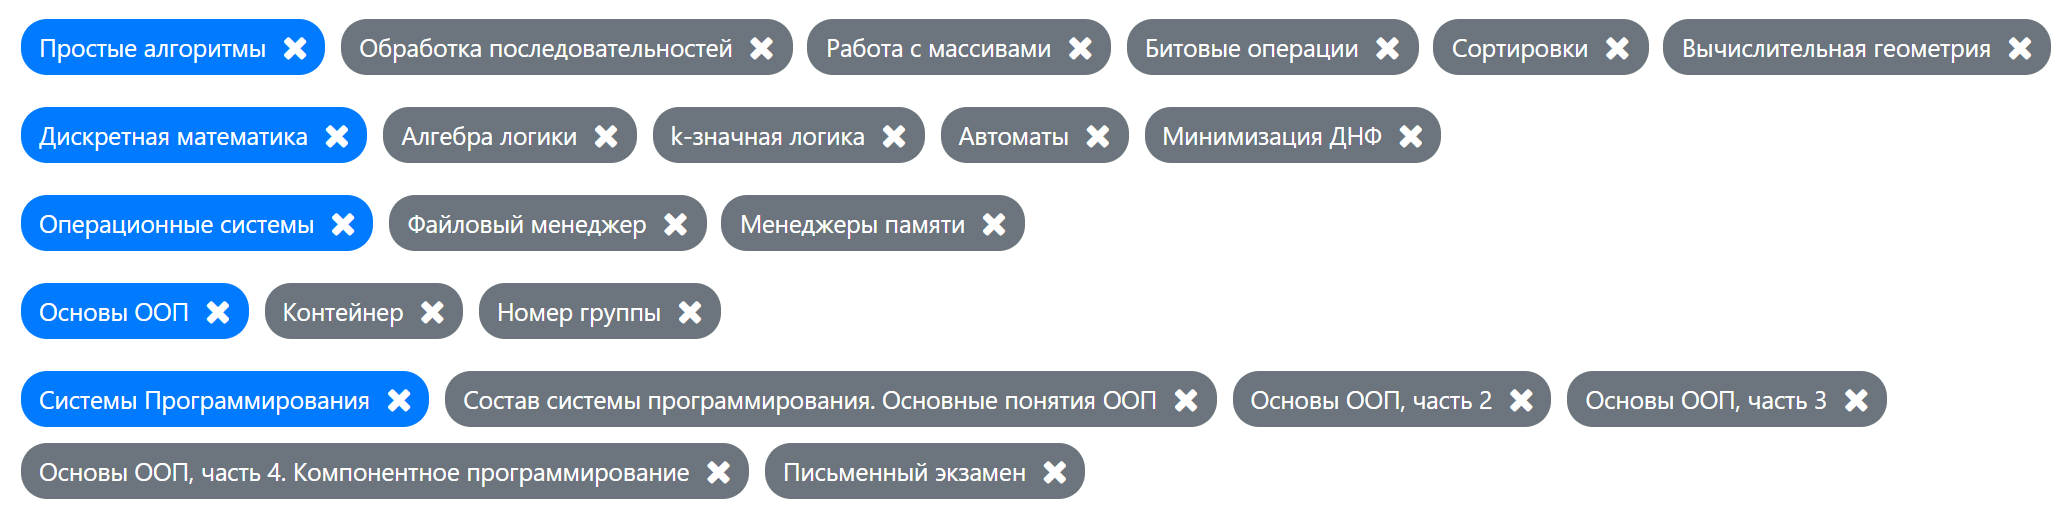
\includegraphics[scale=0.25]{courses-contests-subscriptions}
        \caption{Интерфейс настройки оповещений: список подписок на курсы и разделы}
        \centering
    \end{figure}
\end{frame}

\section{Модуль статистики}
\subsection{Профиль студента}
\subsubsection{Сведения об активности}
\begin{frame}{Сведения об активности студента}
    \begin{figure}
        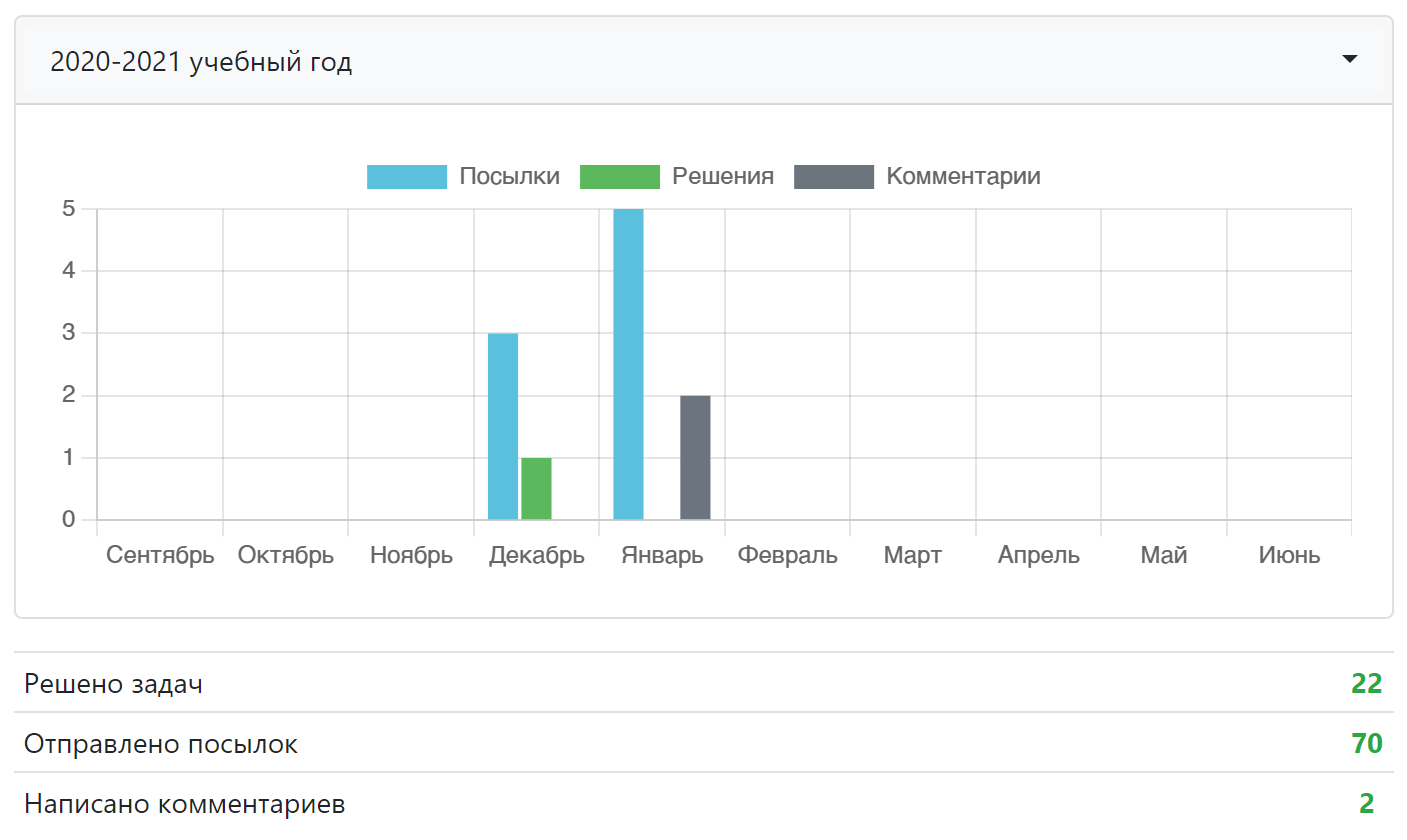
\includegraphics[scale=0.25]{account-activity}
        \caption{Сведения об активности студента}
        \centering
    \end{figure}
\end{frame}
\subsubsection{Результаты курсов}
\begin{frame}{Результаты курсов}
    \begin{figure}
        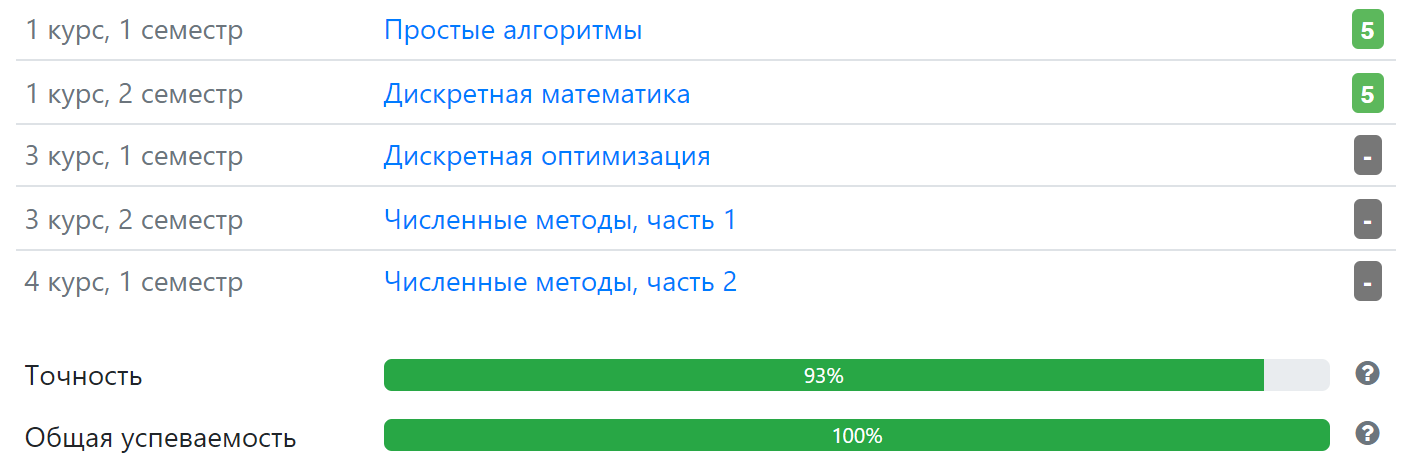
\includegraphics[scale=0.25]{account-courses-results}
        \caption{Результаты курсов}
        \centering
    \end{figure}
\end{frame}
\begin{frame}{Детальные результаты отдельного курса}
    \begin{figure}
        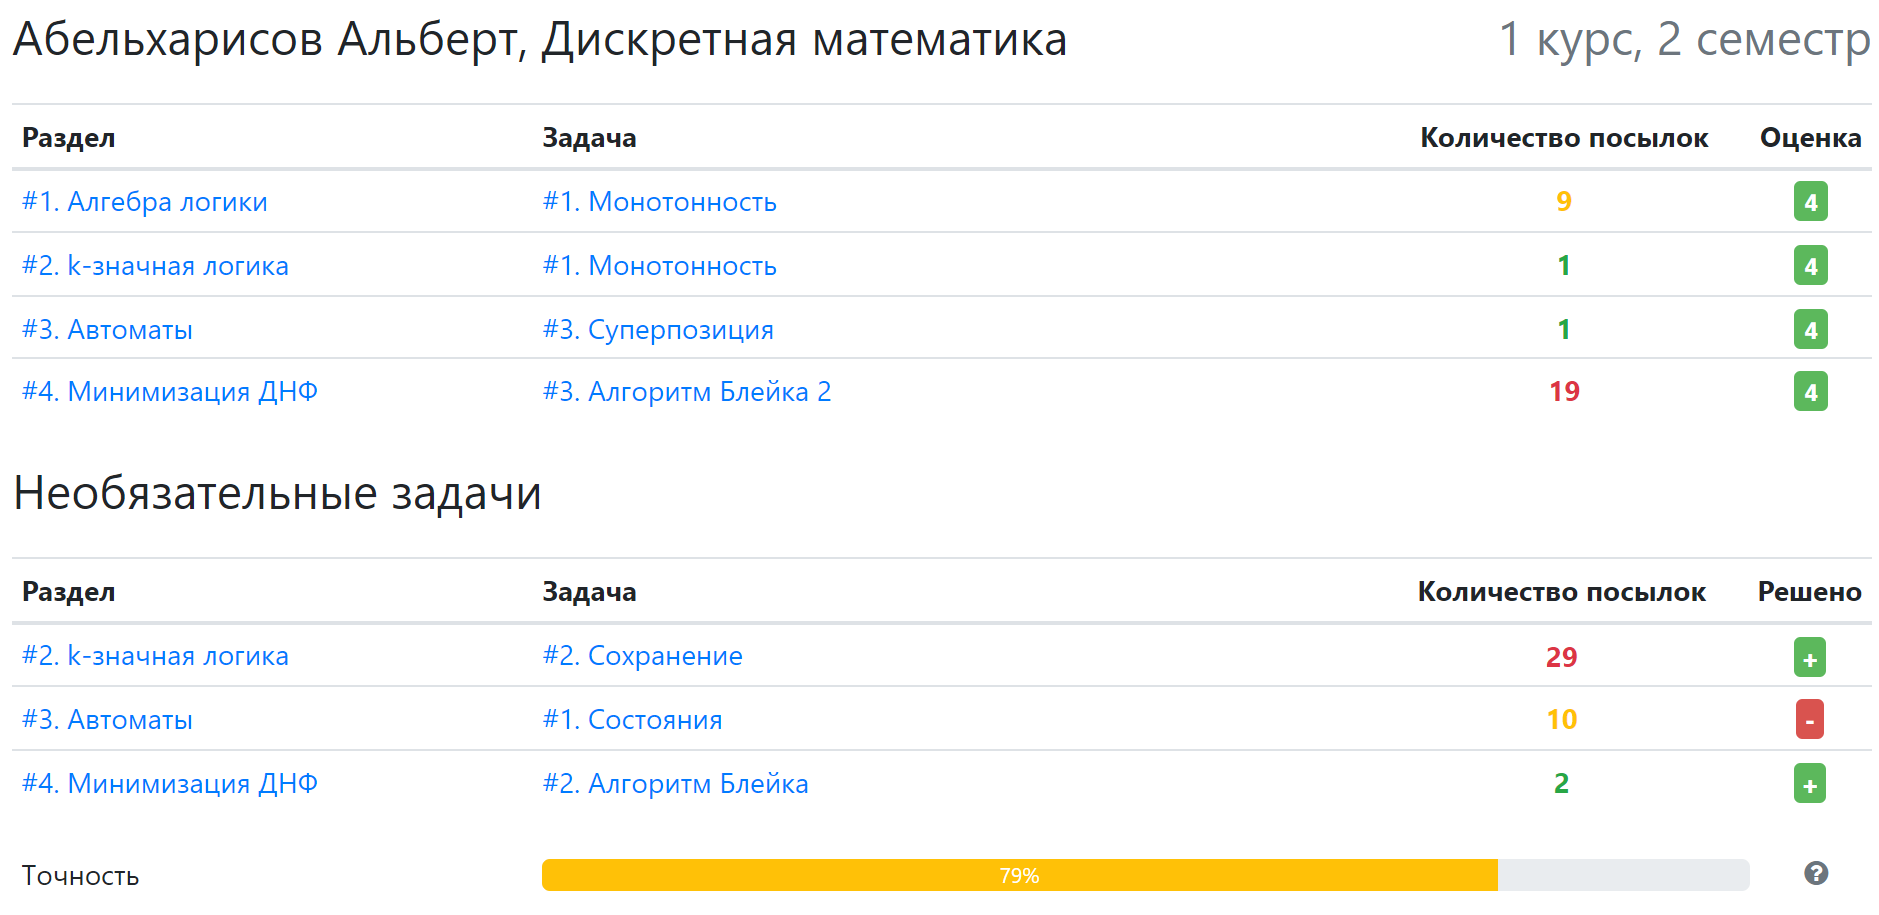
\includegraphics[scale=0.19]{account-course-results}
        \caption{Детальные результаты отдельного курса}
        \centering
    \end{figure}
\end{frame}
\subsubsection{Общая успеваемость и точность}
\begin{frame}{Общая успеваемость и точность студента}
    \begin{itemize}
        \item Общая успеваемость --- средняя оценка студента по пройденным курсам (в процентах)
        \item {
            Точность
            $$\frac{1}{n} \sum_{i=1}^{n} \frac{100\%}{\lceil \frac{C_i}{L_i} \rceil},$$
            где $n$ --- общее количество решенных студентом задач, $C_i$ --- количество посылок к $i$-й задаче до успешной, $L_i$ --- разрешенное количество посылок к $i$-й задаче
        }
    \end{itemize}
\end{frame}
\subsection{Рейтинг студентов}
\begin{frame}{Рейтинг студентов}
    \begin{figure}
        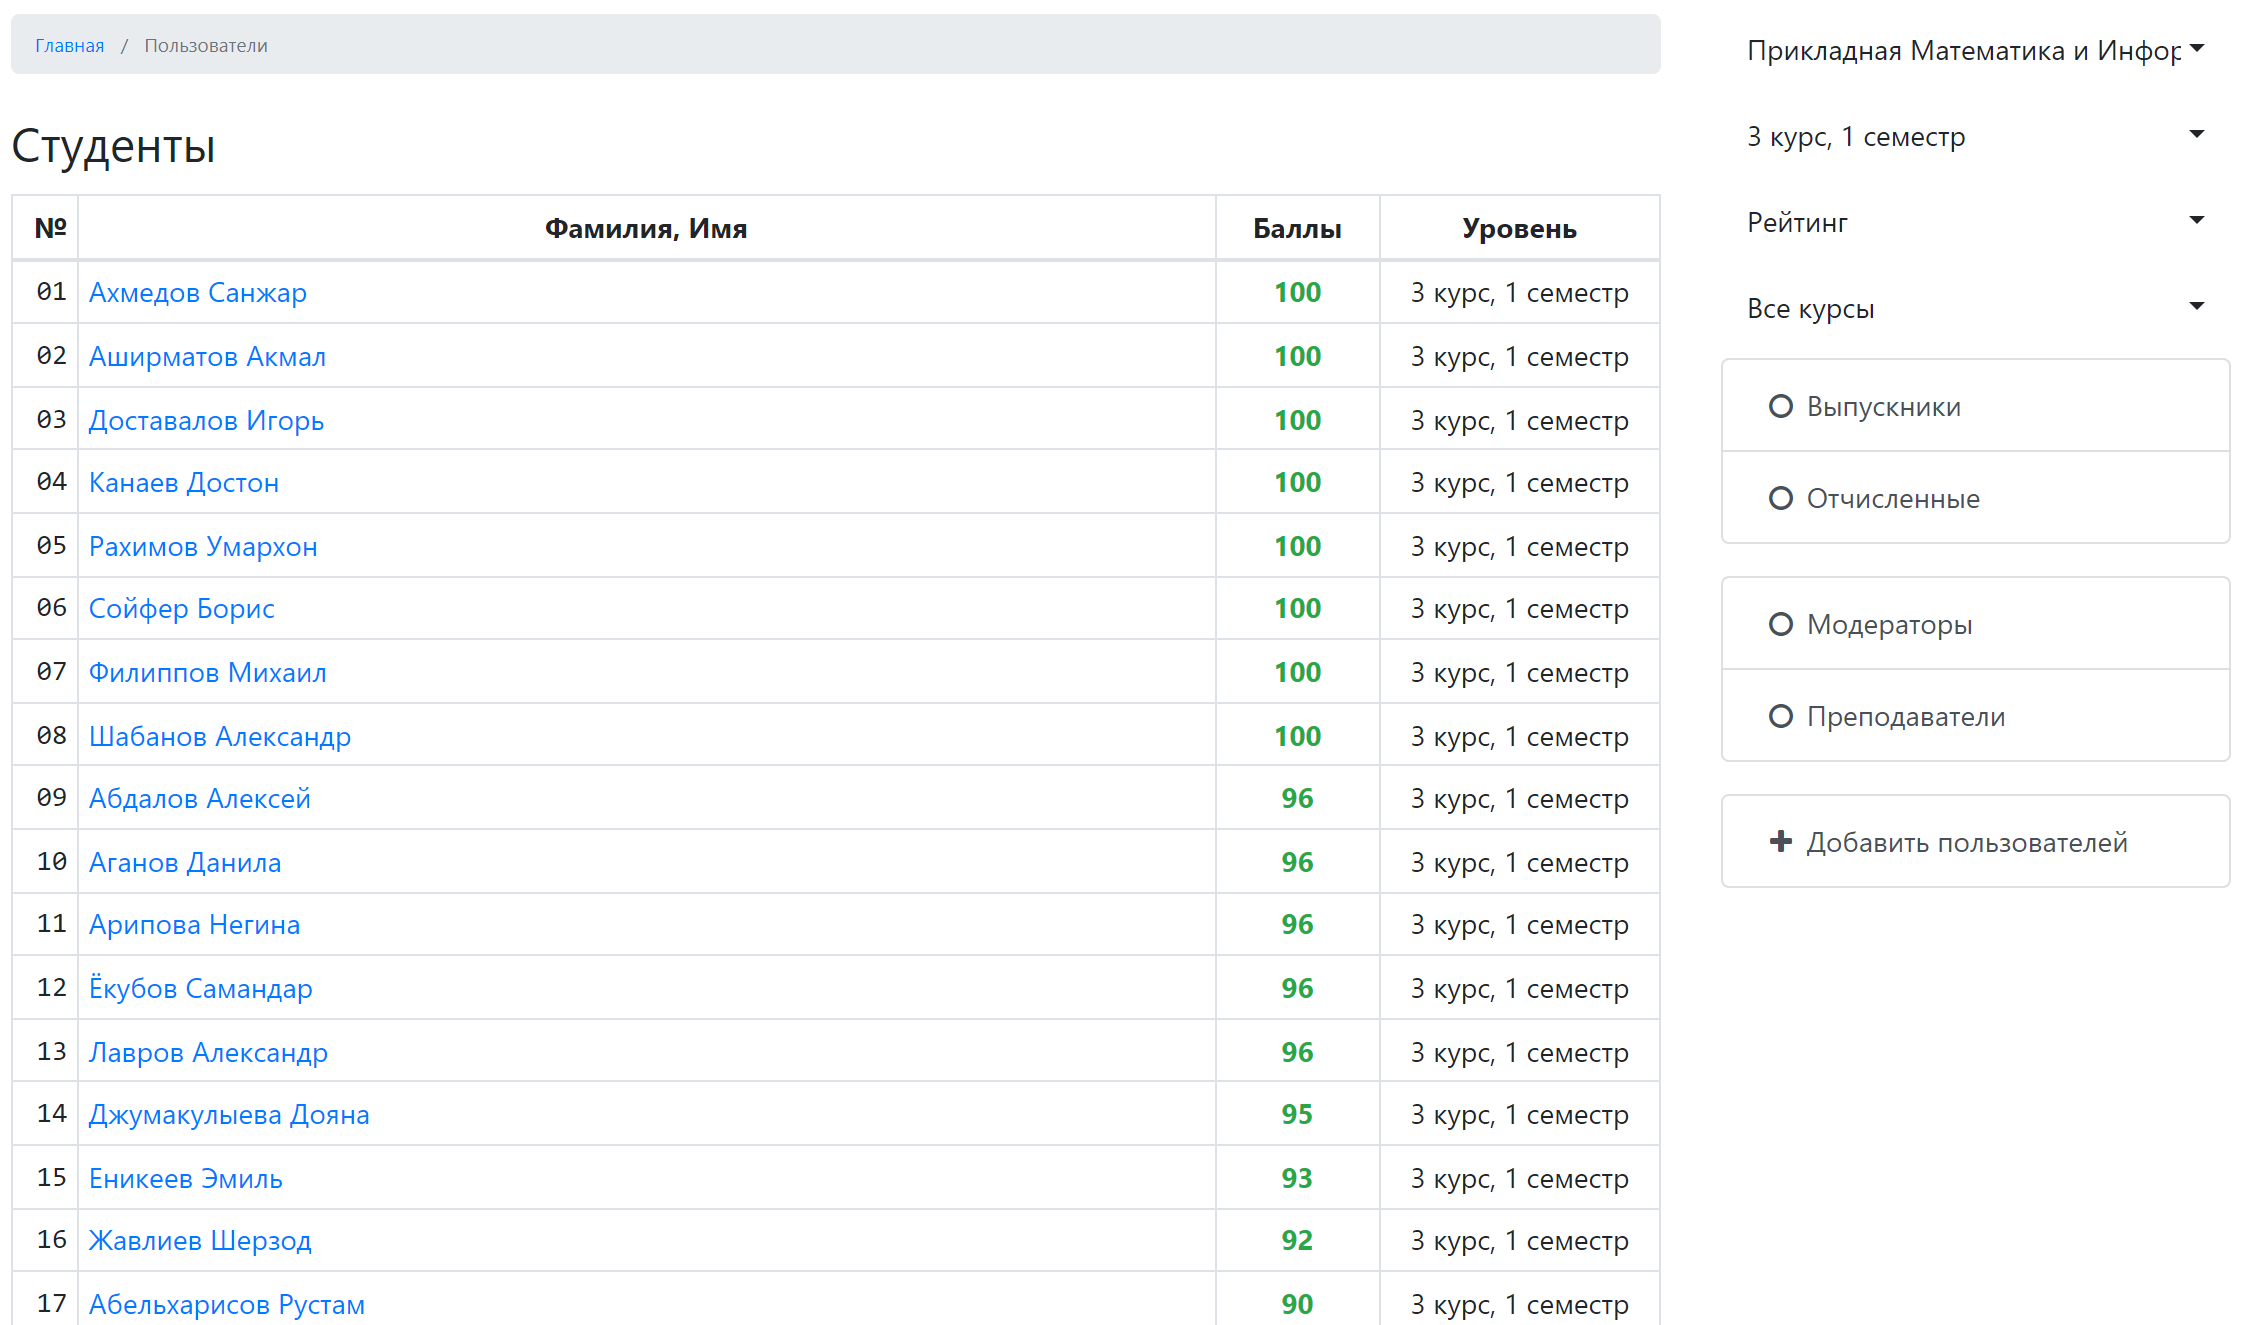
\includegraphics[scale=0.16]{rating}
        \caption{Рейтинг студентов}
        \centering
    \end{figure}
\end{frame}
\subsection{Сведения о сложности курсов}
\begin{frame}{Сведения о сложности курсов}
    \begin{figure}
        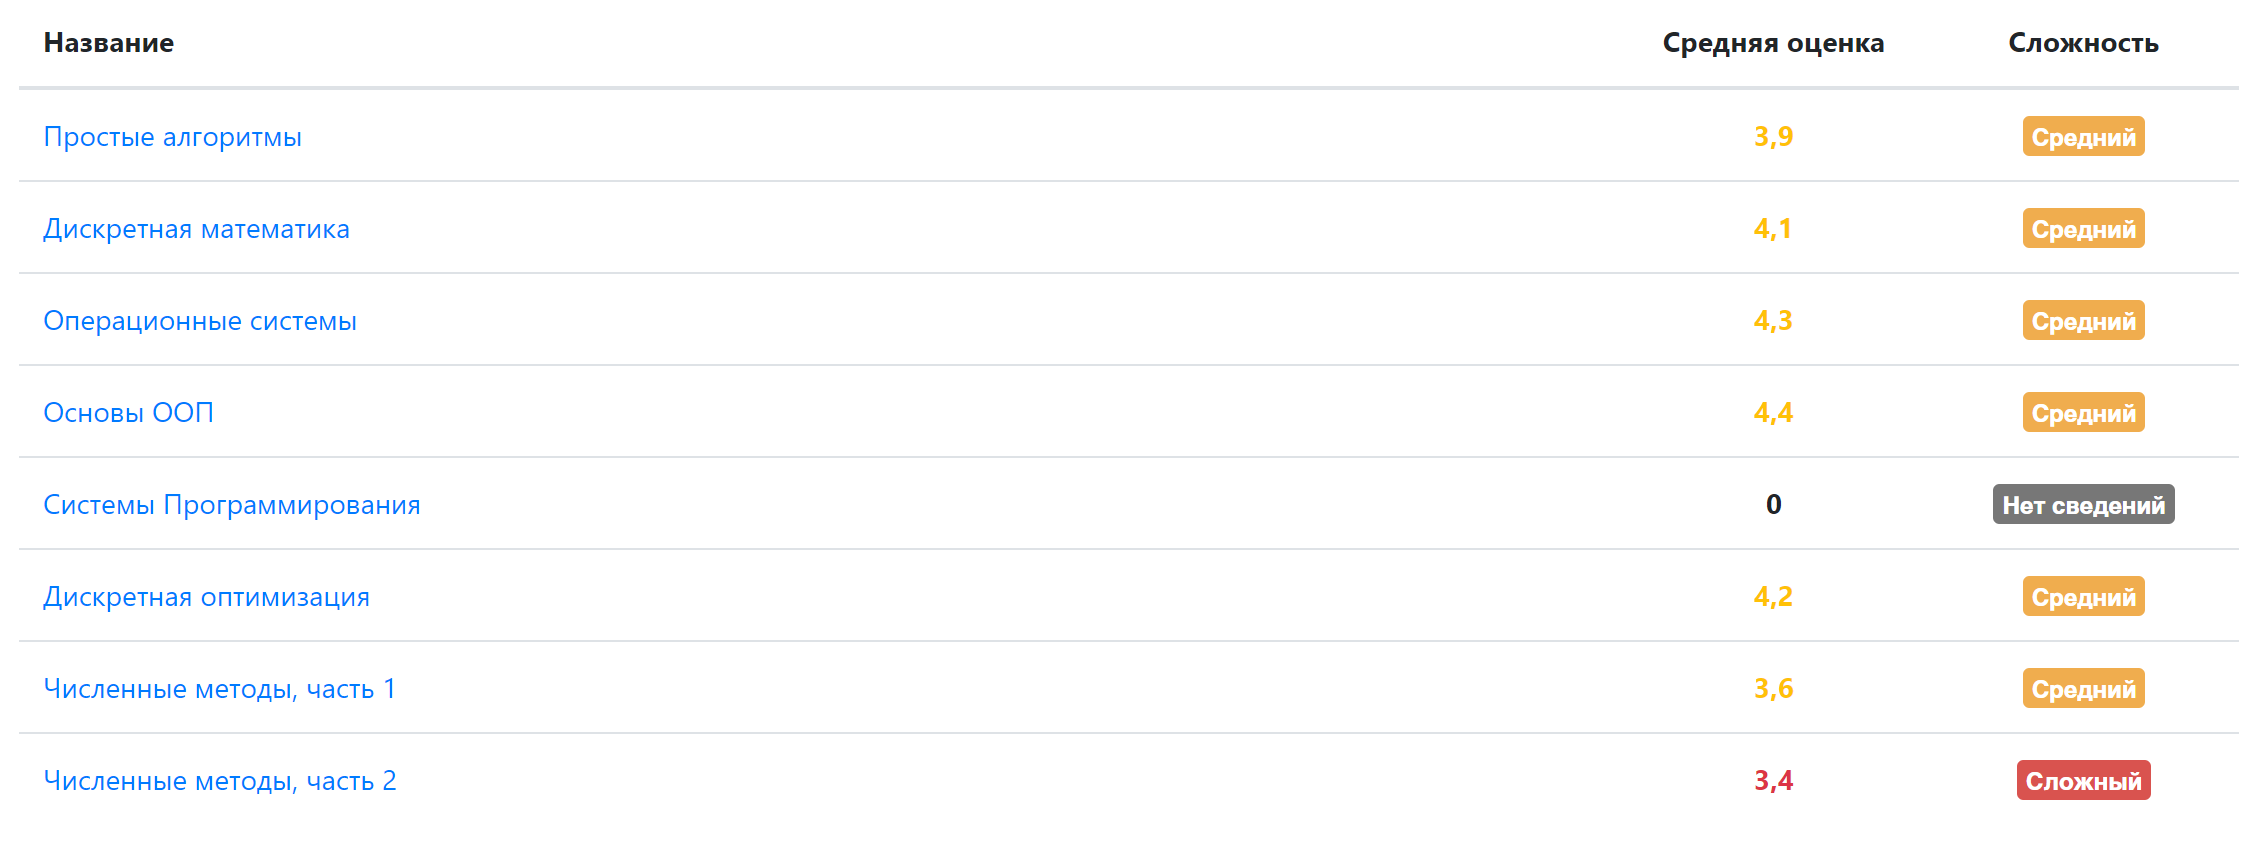
\includegraphics[scale=0.25]{course-difficulty}
        \caption{Сведения о сложности курсов}
        \centering
    \end{figure}
\end{frame}

\section{Раздел помощи}
\begin{frame}{Раздел помощи пользователям}
    \begin{figure}
        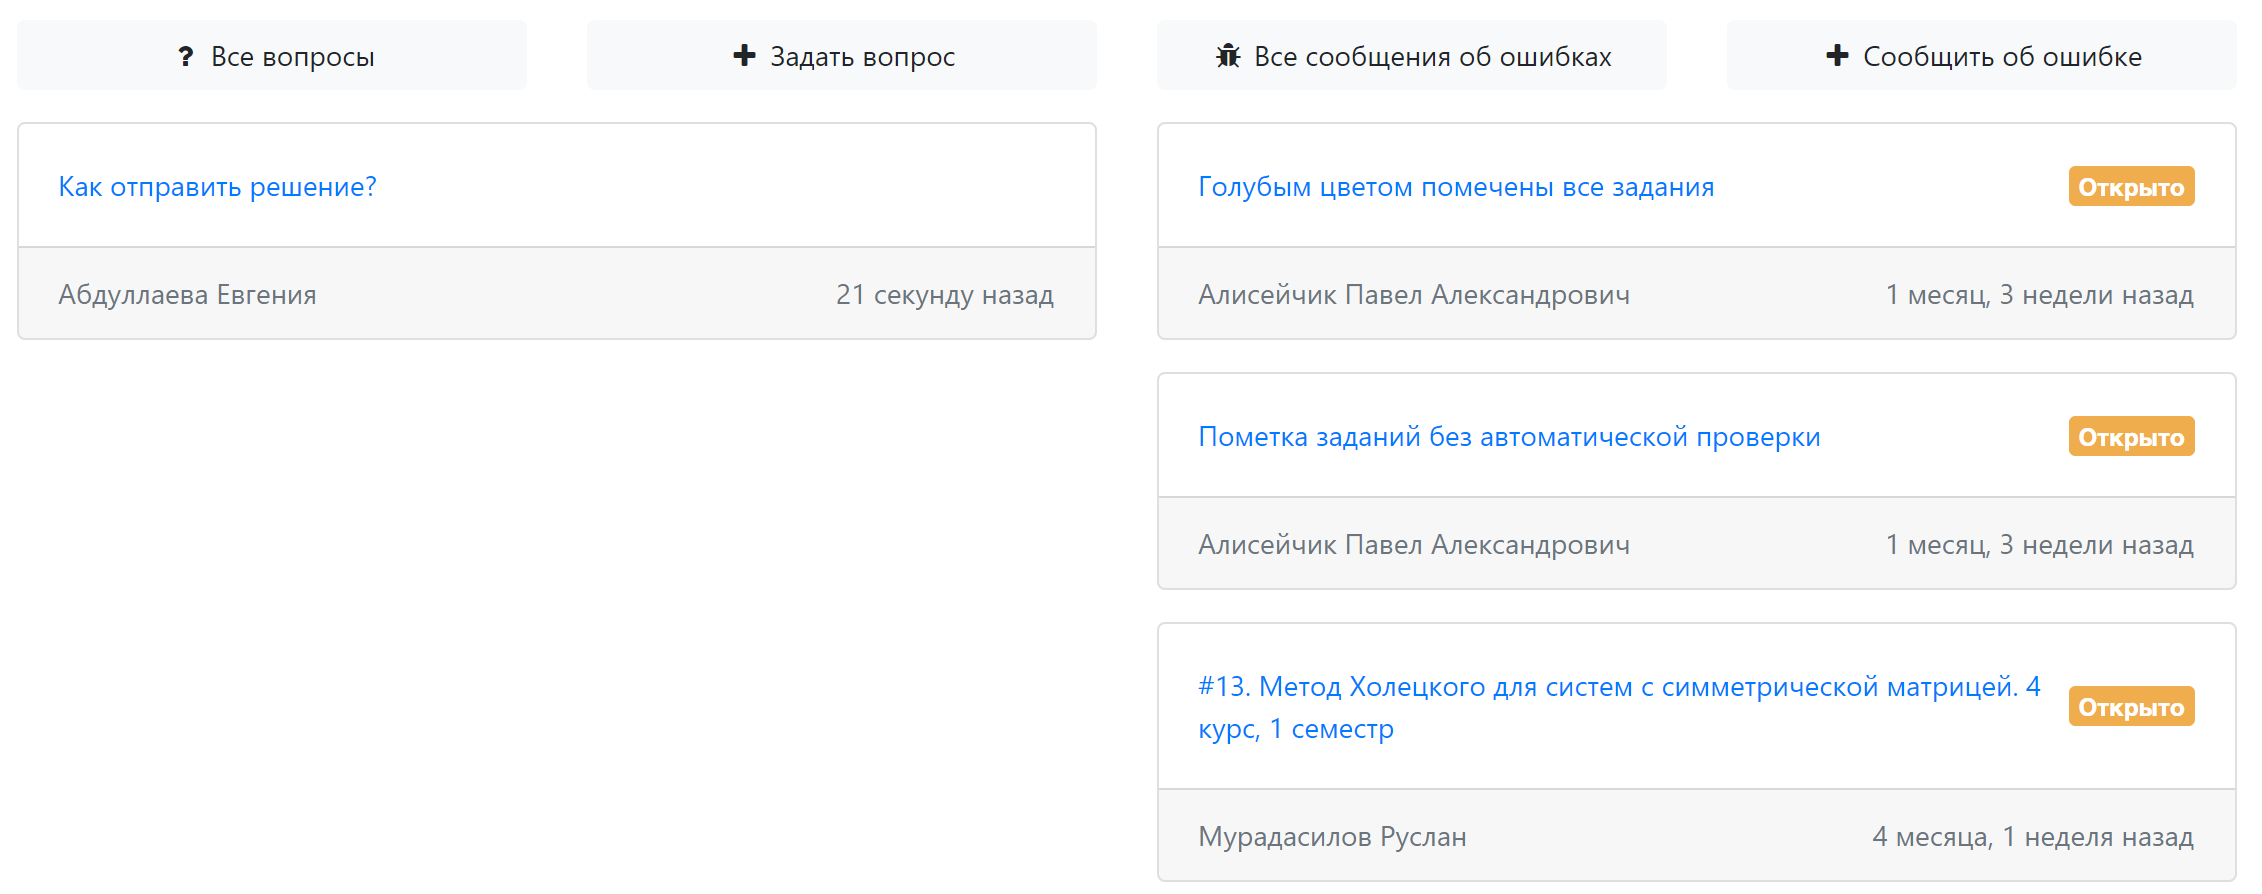
\includegraphics[scale=0.16]{support}
        \caption{Главная страница раздела помощи пользователям}
        \centering
    \end{figure}
\end{frame}
\end{document}